\documentclass[11pt,a4paper]{report}



\usepackage{graphicx}
\usepackage{epstopdf}


\newcommand{\anuga}{\textsc{anuga}}


\newcommand{\inputresults}[1]{\graphicspath{{#1/}}
\section{Dam Break}

Standard dam break test problem. Should show rarefaction fan and shock. 

\subsection{Results}


We should see excellent agreement between the analytical and numerical solutions.

\begin{figure}[h]
\begin{center}
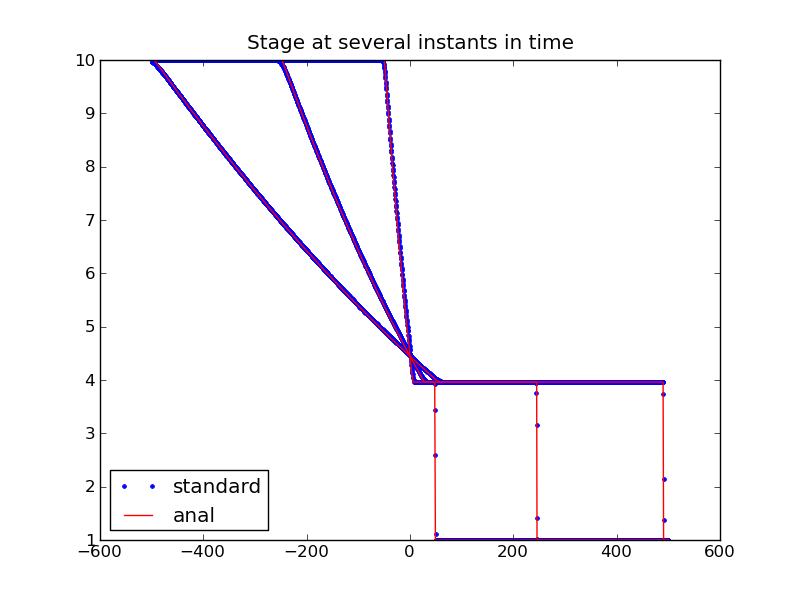
\includegraphics[width=0.9\textwidth]{stage_plot.png}
\end{center}
\caption{Stage results}
\end{figure}


\begin{figure}[h]
\begin{center}
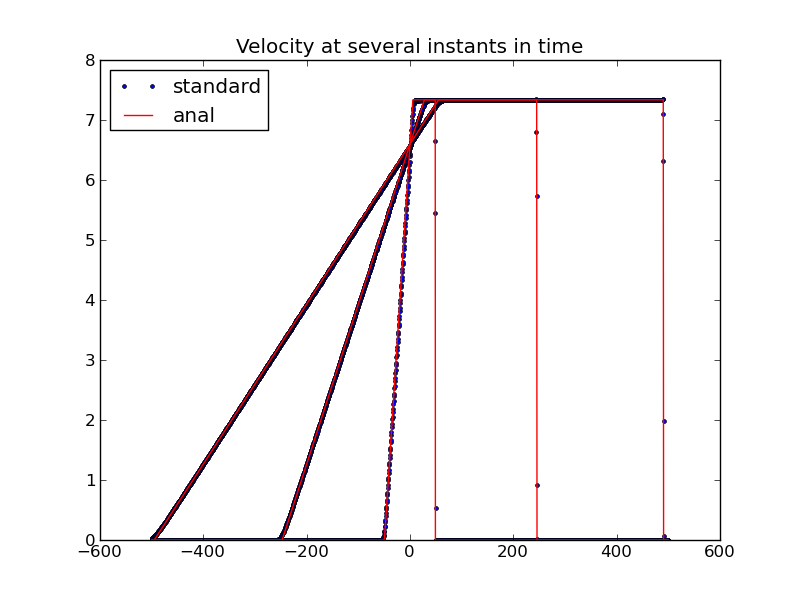
\includegraphics[width=0.9\textwidth]{xvel_plot.png}
\end{center}
\caption{Velocity results}
\end{figure}


\endinput
}

%=========================================
\begin{document} 
%=========================================

%======================
\chapter{Introduction}
%======================

Here we collect the results of running our validation tests. 

\section{Adding New Tests}
To setup a new validation test, create a test directory under the
\textsc{Tests} directory. In that directory there should be the test code, a
\TeX{} file \texttt{results.tex} and a python script
\texttt{produce\_results.py}, which runs the simulation and produces the
outputs. In this \TeX{} file, \texttt{report.tex}, add a line
\begin{verbatim}
\inputresults{Tests/Directory/Name}
\end{verbatim}

%======================
\chapter{Analytical Tests}
%======================

\inputresults{Tests/Analytical/Dam_Break}

\inputresults{Tests/Analytical/runup1}

%======================
\chapter{Experimental Tests}
%======================

\inputresults{Tests/Experimental/Isolated_Building}

%======================
\chapter{Real World Tests}
%======================

\inputresults{Tests/Real_World/Patong}


\end{document}
